\documentclass[11pt,a4paper]{article}

\usepackage{microtype}
\usepackage{graphicx}
\usepackage{listings}
\usepackage{siunitx}
\usepackage{hyperref}
\usepackage{float}

\title{Java Assignment}
\author{Jan van der Lugt}
\date{}

\begin{document}
\maketitle

\section{Introduction}
The report discusses my implementation of a distributed Rubik's cube solver based on the Ibis framework.

Section 2 will provide a design overview of my implementation, section 3 will go through the problems that were identified during the conversation from sequential to distributed code and how they were solved and section 4 will discuss performance results.

\section{Design overview}
My design revolves around a single double-ended queue (deque), which is maintained by the master. The master works on the front of the deque, where it removes a cube and places its children back on the front of the deque. This will cause the cubes with the most work to always be at the end of the deque. In the absence of worker, the master performs the work quite similar to the sequential implementation, with two small differences:
\begin{itemize}
\item The master doesn't use recursion, but use a work deque, which incurs a little more overhead, since adding and removing from a deque is more expensive than a function call. In the case of recursion, however, it is very difficult to steal work from the master.
\item The children are processed in reverse order, since cubes added to the deque are processed in LIFO order. In micro-benchmarks this did not make any difference, which is to be expected because all cubes are explored up to a certain bound anyway.
\end{itemize}
I chose to let the workers steal cubes instead of have the master push them to the workers, since this scheme has the least bookkeeping. Workers always steal from the end of the deque, since these cubes have the most work left to do.

The workers still use the recursive solver, since it is faster and other workers will only steal from the master. In the case of real job-stealing, where every worker can steal from every other worker, they would also have to use a deque, in a similar fashion to the master.

Before the workers can steal work, the master fills the deque with two generations of cubes (in the case of cube of size 3, this amounts to 144 cubes). Future work could include setting this number dynamically based on the number of workers. In this filling phase, the master also works from the end of the deque, so the deque will have cubes with equal and relatively large amounts of work.

\section{Problems during implementation}

\subsection{Concurrency and synchronization}
In the presence of $n$ workers, there are multiple threads active in the master: one main thread and up to $n$ threads of workers requesting work. In order to make sure threads only steal work when they are supposed to and wait when necessary, several mechanisms are used to make sure everything works according to plan:
\begin{itemize}
\item A \emph{status} enum which denotes the current phase of the computation. This can be initialization, filling deque, processing deque, deque empty, waiting for workers or done.
\item `synchronized' statements are used to make sure two threads are not accessing the deque at the same time. They also make sure that the status enum can be changed atomically based on an observation of the deque (for example when it is empty).
\item notify(), notifyAll() and wait() calls are made to sleep when this is necessary (for example when workers need to wait until work is available).
\item AtomicIntegers are used to store the number of solutions and the number of workers the master is still waiting for.
\end{itemize}

\subsection{Handling SendPorts on the master}
The master has to have SendPorts to all workers open to avoid having to create a new connection upon every incoming request. To do this, the master implements \emph{ReceivePortConnectUpcall}, so it creates a SendPort whenever a worker connects to it ReceivePort. These SendPorts are stored in a HashMap, so they can be retrieved later based on an IbisIdentifier.

\subsection{Termination}
Because I was having some trouble with Ibis termination mechanism, which is probably caused by not having an example available explaining how to use it, I created a very simple termination mechanism:

Every cube that is sent from the master to the worker, is preceded by a boolean. Normally this boolean is false, but when the master decides it is time to terminate, it sends a true, signaling the workers to quit.

Everyone then closes their SendPorts and then their ReceivePorts (since closing a ReceivePort blocks if there is still a SendPort connected to it).

\section{Performance results}
To test the performance, I tested three types of cubes, in order of complexity:
\begin{enumerate}
\item A cube of size 3 with 11 twists (2 solutions in 7 steps)
\item A cube of size 3 with 12 twists (4 solutions in 8 steps)
\item A cube of size 4 with 11 twists (2 solutions in 7 steps)
\end{enumerate}
All of these cubes were created with seed 0. Since all cubes up to a certain bound are searched for solutions, the seed value does not matter very much, as long as the minimum number of steps in the solution is the same. The numbers below are in seconds and averaged over 3 runs. \\

\begin{tabular}{ | l | S | S | S | S | S | S | }
	\hline
	\textbf{Cube type} & \textbf{Sequential} & \textbf{IPL 1} & \textbf{IPL 2} & \textbf{IPL 4} & \textbf{IPL 8} & \textbf{IPL 16} \\
	\hline                       
	Size 3, 11 twists & 10.5 & 13.2 & 6.2 & 3.2 & 1.8 & 1.2 \\
	\hline
	Size 3, 12 twists & 122.6 & 159.8 & 69.8 & 33.4 & 16.7 & 8.9 \\
	\hline
	Size 4, 11 twists & 209.5 & 245.6 & 113.2 & 54.5 & 27.0 & 13.5 \\
	\hline
\end{tabular} \\

As can be seen in the graphs on the next page, some of the speedups are superlinear. This can be explained by the fact that the workers use a more efficient solver, the one based on recursion. The more workers, the less work the less efficient solver of the master has to do.

Implementing work stealing between workers would probably not help much, since all cubes with an equal number of twists and an equal bound have the same amount of work. For puzzles that do not have such a predictable amount of work, work stealing between workers would be more beneficial.

\begin{figure}[h]
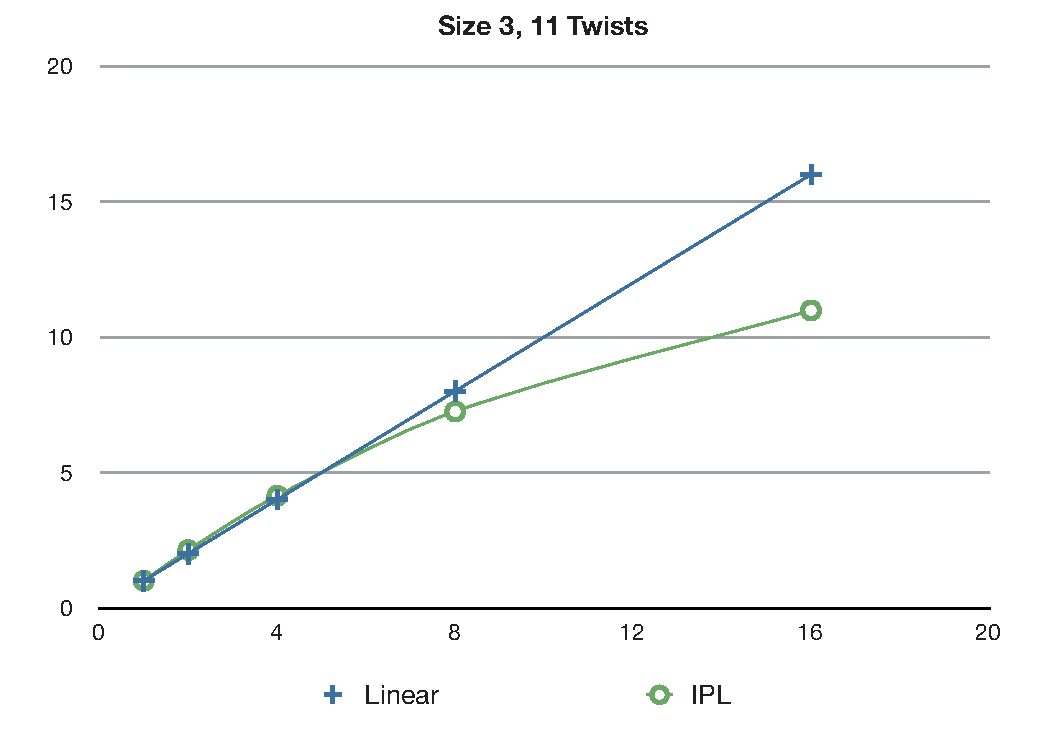
\includegraphics[scale=0.5]{figures/3-11.pdf}
\end{figure}

\begin{figure}[h]
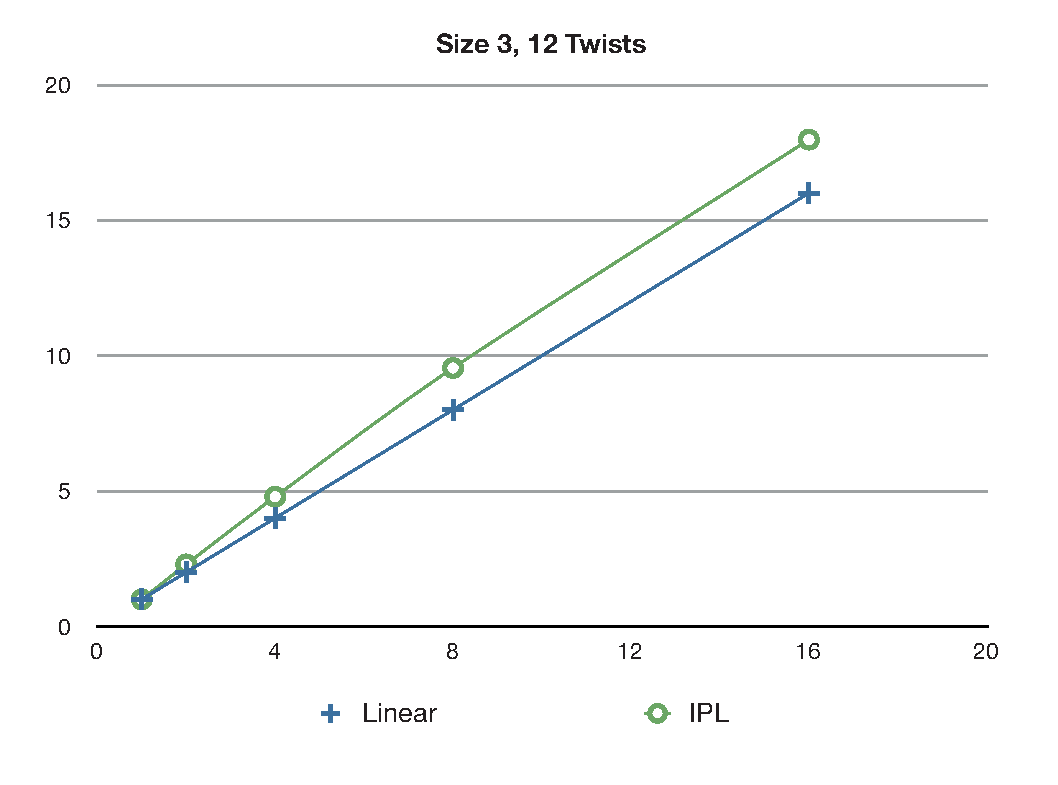
\includegraphics[scale=0.5]{figures/3-12.pdf}
\end{figure}

\begin{figure}[h]
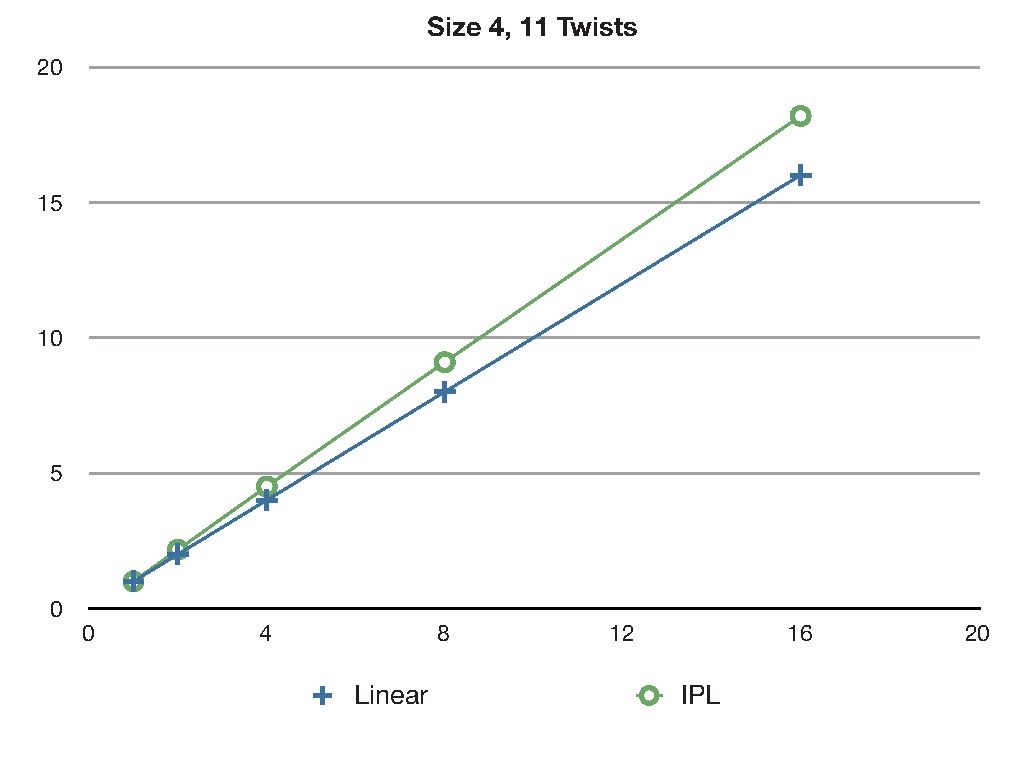
\includegraphics[scale=0.5]{figures/4-11.pdf}
\end{figure}


\end{document}
